\documentclass[aspectratio=169]{beamer}
%-----------------------------------------------------------------------
%%%% packages y comandos personales %%%%
\usepackage[utf8]{inputenc}
\usepackage[spanish]{babel}
\usepackage{alltt}
\usepackage{hyperref}
\usepackage[Symbol]{upgreek}
\usepackage{latexsym}
\usepackage{amsmath,amssymb,amsfonts}
\usepackage{graphics,epsfig,subfigure}
\usepackage{url}
\usepackage{caption}
\usepackage{multimedia}
\usepackage{slashbox}
\usepackage{media9}
\usepackage[Symbol]{upgreek}
\usepackage{MnSymbol}
\usepackage{tikz}
\usepackage{palatino}
\usepackage{color}
\usepackage[skins,theorems]{tcolorbox}
\usepackage[Symbol]{upgreek}
\usepackage{MnSymbol}
\usepackage{geometry}
\usepackage{tabularx}
\usepackage{arydshln}
\usepackage{textcomp}
\usepackage{marvosym}
\usepackage{lipsum}
\usepackage{pifont}
\usepackage{algorithmic}
\usepackage{longtable}
\usepackage{lscape}
\usepackage{booktabs}
\usepackage{bm}
\usepackage{enumitem}
%-----------------------------------------------------------------------
\newtheorem{teorema}{Teorema}
\newtheorem{ejemplo}{Ejemplo}
\newtheorem{definicion}{Definici\'on}
\newtheorem{corolario}{Corolario}
\newtheorem{prueba}{Prueba}
%-----------------------------------------------------------------------
\mode<presentation>
{
  \usetheme{Boadilla}               % try: Default, Boadilla, Darmstadt, Madrid, Warsaw, Montpellier ...
  \usecolortheme{whale}             % try: whale albatross, beaver, crane, ...
  \usefonttheme{professionalfonts}  % intente serif, structurebold, ...
  \setbeamertemplate{navigation symbols}{}
  \setbeamertemplate{caption}[numbered]
  \usefonttheme{serif}
  \setbeamertemplate{blocks}[rounded][shadow=true]
}
%-----------------------------------------------------------------------
\title[TP1]{Desarrollo del TP1: Métodos de Búsqueda}
\author[Grupo ITBA No. 8]{Mauro Baquero-Su\'arez \inst{1} \and Dario Alejandro Peñaloza \inst{1} \and Lucas Miguel Biolley \inst{1} \and Mariano Pérez Mosquera \inst{1}}
\institute[ITBA]{\inst{1} Instituto Tecnológico de Buenos Aires (ITBA)}
\date[\today]{
\includegraphics[scale=.034]{Figures/ITBA_Logo.png}}
%-----------------------------------------------------------------------
% Define colors:
\definecolor{JadeGreen}{RGB}{0,128,168}
\definecolor{ParakeetGreen}{RGB}{34,177,76}
\definecolor{UBCblue}{rgb}{0.04706, 0.15725, 0.296667} % UBC Blue (primary)
\definecolor{UBCgrey}{rgb}{0.3686, 0.5255, 0.6235} % UBC Grey (secondary)
% Beamer colors:
\setbeamercolor{palette primary}{bg=UBCblue,fg=white}
\setbeamercolor{palette secondary}{bg=UBCgrey,fg=white}
\setbeamercolor{palette tertiary}{bg=UBCblue,fg=white}
\setbeamercolor{palette quaternary}{bg=UBCblue,fg=white}
\setbeamercolor{structure}{fg=UBCblue} % itemize, enumerate, etc
\setbeamercolor{section in toc}{fg=UBCblue} % TOC sections
% Override palette coloring with secondary
\setbeamercolor{subsection in head/foot}{bg=UBCgrey,fg=white}
% Color boxes:
\tcbset{myinner/.style={no shadow,shrink tight,extrude by=1mm,colframe=blue,colback=blue!5!white,
  boxrule=0.6pt,frame style={opacity=0.25},interior style={opacity=0.5}}}
%-----------------------------------------------------------------------
\begin{document}
\spanishdecimal{.}
\maketitle
%-----------------------------------------------------------------------
\section{Introducción}
%-----------------------------------------------------------------------
\begin{frame}
\frametitle{Introducción}
El objetivo de este TP es implementar y evaluar diferentes métodos de búsqueda para la solución de diferentes problemas que requieren agentes inteligentes.
\end{frame}
%-----------------------------------------------------------------------
\section{Desarrollo de los Ejercicios}
%-----------------------------------------------------------------------
\begin{frame}
\frametitle{Ejercicio No. 1: 8-Puzzle}
\framesubtitle{Estructura de Estado (SS)}
\begin{columns}
\column{.18\textwidth}
\hspace{-.25cm}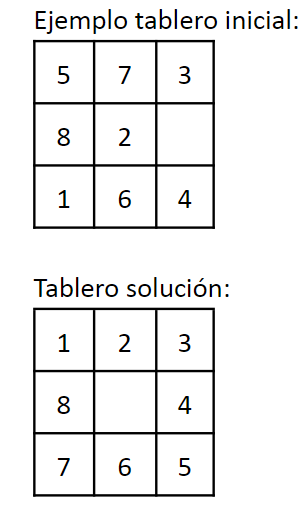
\includegraphics[scale=.55]{Figures/8-Puzzle.png}
\column{.8\textwidth}
\begin{definicion}[Estructura de Estado (SS)]
En este ambiente discreto y determinístico, definiríamos SS de manera
generalizada dentro del dominio $D\subset\mathbb{Z}_{+}$ tal que,
\begin{equation*}
x_i(k) = \left\{r_i(k),c_i(k)\right\} \in \mathbb{Z}_{+}^{\{n^2-1\times2\}}
\end{equation*}
corresponde al conjunto de posiciones de cada $i$ ésima ficha para $i=\left\{0,1,\ldots,n^2-1\right\}$. Las
posiciones estarán establecidas como el No. de filas $1\!\leq\!r_i(k)\!\leq\!n$ y el No. de
columnas $1\!\leq\!c_i(k)\!\leq\!n$ de la matriz que se forma con estas variables en el instante $k$.
\end{definicion}
\begin{itemize}
\item Para el caso del 8-Puzzle: \textcolor{blue}{$n = 3$}.
\end{itemize}
\end{columns}
\end{frame}
%-----------------------------------------------------------------------
\begin{frame}
\frametitle{Ejercicio No. 1: 8-Puzzle}
\framesubtitle{Heurísticas no Triviales}
\begin{definicion}[Función Sucesora]
Sea $U(k)$ la función sucesora, correspondiente al conjunto de posibles movimientos de $x_0(k)$ hacia:
\begin{columns}
\column{.58\textwidth}
\vspace{-.3cm}\begin{equation*}
U\!(k+1) \!=\! \left\{\begin{array}{c}
\!\!u_1(k\!+\!1) \!=\! \overbrace{\left(r_0(k)\!-\!1,c_0(k)\right)}^{x_0(k)\text{ para Arriba}}, \hspace{.15cm} \forall r_0(k)\!>\!1\!\! \\
\!\!u_2(k\!+\!1) \!=\! \overbrace{\left(r_0(k)\!+\!1,c_0(k)\right)}^{x_0(k)\text{ para Abajo}}, \hspace{.15cm} \forall r_0(k)\!<\!n\!\! \\
\!\!u_3(k\!+\!1) \!=\! \overbrace{\left(r_0(k),c_0(k)\!-\!1\right)}^{x_0(k)\text{ para Izquierda}}, \hspace{.15cm} \forall c_0(k)\!>\!1\!\! \\
\!\!u_4(k\!+\!1) \!=\! \overbrace{\left(r_0(k),c_0(k)\!+\!1\right)}^{x_0(k)\text{ para Derecha}}, \hspace{.15cm} \forall c_0(k)\!<\!n\!\!
\end{array}\right\},
\end{equation*}
\column{.42\textwidth}
permutando la posición del $x_j(k)$ que coincide con el cambio aplicado a $x_0(k)$.
\end{columns}
\end{definicion}
\end{frame}
%-----------------------------------------------------------------------
\begin{frame}
\frametitle{Ejercicio No. 1: 8-Puzzle}
\framesubtitle{Heurísticas no Triviales}
Teniendo en cuenta $U\!(k+1)$, se pueden definir heurísticas que permitan seleccionar el movimiento sucesor $u_m(k\!+\!1)$
más viable para llegar a la solución del estado objetivo $x_i^*\!=\!\left(r_i^*,c_i^*\right)$. Entonces, definimos la primera heurística:
\begin{definicion}[Heurística de la Norma Euclideana (HNE)]
Sea $^m\!x_i(k\!+\!1)$ el resultado de aplicar $u_m(k\!+\!1)$ para cada $m\!=\!\left\{1,2,3,4\right\}$, entonces de define
HNE como:
\begin{equation*}
h_1(k\!+\!1) := \underset{m}{\mathrm{arg\,min}}\sum_{i=0}^{n^2-1}\!\sqrt{\left[^mr_i(k\!+\!1) - r_i^*\right]^2 + \left[^mc_i(k\!+\!1) - c_i^*\right]^2},
\end{equation*}
y la selección del nuevo $x_i(k\!+\!1)$ sería:
\begin{equation*}
x_i(k\!+\!1) = \left\{^m\!x_i(k\!+\!1) \hspace{.2cm} | \hspace{.2cm} h_1(k\!+\!1)>0\right\}.
\end{equation*}
\end{definicion}
\end{frame}
%-----------------------------------------------------------------------
\begin{frame}
\frametitle{Ejercicio No. 1: 8-Puzzle}
\framesubtitle{Heurísticas no Triviales}
y la segunda heurística:
\begin{definicion}[Heurística Matricial (HM)]
Sea $^m\!x_i(k\!+\!1)$ el resultado de aplicar $u_m(k\!+\!1)$ para cada $m\!=\!\left\{1,2,3,4\right\}$ y $^m\!M\!(k\!+\!1)\!:=\!i_{r,c}^{+}$
la matriz formada por las fichas $i$ del tablero, en sus posiciones $r_i(k\!+\!1)$ y $c_i(k\!+\!1)$. Entonces definimos HM como:
\begin{equation*}
h_2(k\!+\!1) := \underset{m}{\mathrm{arg\,min}}\left|\det\!\left\{^m\!M\!(k\!+\!1)\right\} - \det\!\left\{M^*\right\}\right|,
\end{equation*}
donde $\det\{\cdot\}$ es el determinante de la matriz y $M^*\!:=\!i_{r,c}^*$ es la matriz objetivo formada por la fichas en las posiciones deseadas $r_i^*$ y $c_i^*$. Luego, la selección del nuevo $x_i(k\!+\!1)$ sería:
\begin{equation*}
x_i(k\!+\!1) = \left\{^m\!x_i(k\!+\!1) \hspace{.2cm} | \hspace{.2cm} h_2(k\!+\!1)>0\right\}.
\end{equation*}
\end{definicion}
\end{frame}
%-----------------------------------------------------------------------
\begin{frame}
\frametitle{Ejercicio No. 1: 8-Puzzle}
\framesubtitle{Método de búsqueda escogido: Global Greedy Search (GGS)}
\begin{itemize}
\item Es un método de búsqueda informado que puede tomar los datos que se tienen del tablero.
\item No requiere estimar costo en las acciones. En este caso el costo para cada movimiento de $x_0$ es el mismo,
sea para arriba, abajo, derecha ó izquierda.
\item Se requiere evaluación de repetición de estados.
\item Es eficiente para este caso, especialmente para $n=3$.
\end{itemize}
\end{frame}
%-----------------------------------------------------------------------
\begin{frame}
\frametitle{Ejercicio No. 1: 8-Puzzle}
\framesubtitle{Heurística escogida: Distancia Manhattam}
\begin{itemize}
\item Es un cálculo que se ejecuta muy rápido.
\item Es admisible.
\item Es sencillo de implementar.
\end{itemize}
\end{frame}
%-----------------------------------------------------------------------
\begin{frame}
\frametitle{Ejercicio No. 2: Sokoban}
\framesubtitle{Estructura de Estado (SS)}
\begin{definicion}[Estructura de Estado (SS)]
La SS de este problema se definirá como la posición de los tres elementos principales (personaje, caja y objetivo)
de modo que: 
\begin{equation*}
x_i(k) = \left\{r_i(k),c_i(k)\right\} \text{ para } i = \left\{1,2,3\right\},
\end{equation*}
donde $i$ representa a cada uno de los tres elementos, y sus posiciones estarán establecidas como el No. de filas $1\!\leq\!r_i(k)\!\leq\!n$ y el No. de
columnas $1\!\leq\!c_i(k)\!\leq\!n$ de la matriz de dimensión $n\!\times\!n$, correspondiente al mapa en el instante $k$.
\end{definicion}
\end{frame}
%-----------------------------------------------------------------------
\section{Conclusiones}
%-----------------------------------------------------------------------
\begin{frame}
\frametitle{Conclusiones}
\begin{itemize}
\item ....\vspace{.25cm}
\item ....
\end{itemize}
\end{frame}
%-----------------------------------------------------------------------
\begin{frame}
\frametitle{Final de la presentación}

\Huge Gracias...!
\end{frame}
%-----------------------------------------------------------------------
\end{document}
